%%%%%%%%%%%%%%%%%%%%%%%%%%%%%%%%%%%%%%%%%%%%%%%%%%%%%%%%%%%%%%%%%%%%%%%
%%%%%%%%%%%%%%%%%%%%%%%%%%%%%%%%%%%%%%%%%%%%%%%%%%%%%%%%%%%%%%%%%%%%%%%
%%%%%                                                                 %
%%%%%     <file_name>.tex                                             %
%%%%%                                                                 %
%%%%% Author:      <author>                                           %
%%%%% Created:     <date>                                             %
%%%%% Description: <description>                                      %
%%%%%                                                                 %
%%%%%%%%%%%%%%%%%%%%%%%%%%%%%%%%%%%%%%%%%%%%%%%%%%%%%%%%%%%%%%%%%%%%%%%
%%%%%%%%%%%%%%%%%%%%%%%%%%%%%%%%%%%%%%%%%%%%%%%%%%%%%%%%%%%%%%%%%%%%%%%


\chapter{Design Implementation}


\section { Porting Halide to new targets}
    Halide programs rely on the \gls{llvm} library to generate compiled code for the desired targets. To build the Halide library, we first need to build \gls{llvm} with the correct flags and add the support for the building machine.
    As the \gls{hero} toolchain already has a build of this compiler, we can use it to compile Halide, but the \texttt{-DBUILD\_SHARED\_LIBS} flag has to be disabled, as Halide does not support shared libraries.
    We added a \texttt{make} target to to main \texttt{Makefile} of the project, to simplify the installation process.

    Once the installation process was complete, we worked on porting Halide to \gls{hero} on the hardware simulation.
    The hardware simulation runs an \gls{rtl} simulation of a \gls{pulp} cluster configured with eight cores. This platform is easier to work on as it does not require any specific hardware (\gls{fpga}) and uses one of the cluster's core as the host of the system.

    %%%%%%%%%%%%%
    \section{Compilation Workflow}

\begin{figure}[H]
\dirtree{%
    .1 halide-examples/.
    .2 common/.
    .3 defaultHalide.mk.
    .2 myApp/.
    .3 main.c.
    .3 Makefile.
    .3 lib/.
    .4 halidePipeline.cpp.
    }
    \caption{Directory structure for Halide applications.}
    \label{Fig:DirectoryStructure}
\end{figure}



    Every application follows the directory structure described in Figure~\ref{Fig:DirectoryStructure}, the \texttt{common} folder is shared between all the applications and contains a common \texttt{Makefile} that will be included in every application's \texttt{Makefile}.
    The source code is split between two files, the pipeline generator in the \texttt{lib/} folder, and the main \gls{hero} application.
    The pipeline generator uses Halide to generate the pipeline object file which will be used during the compilation of the application.

\begin{figure}[h]
    \centering
    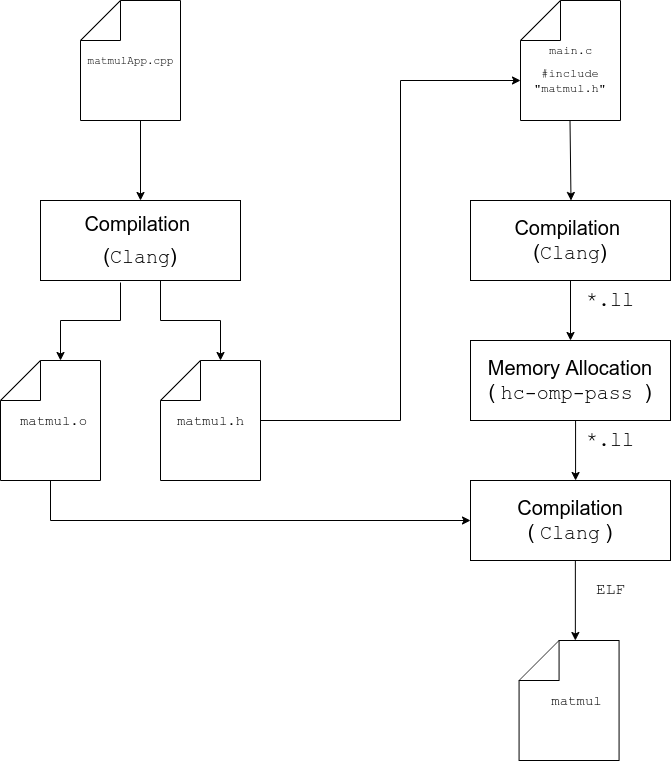
\includegraphics[width=.5\textwidth]{./figures_raw/compilationWorkflow.png}
    \caption{Compilation Workflow for an Halide Application.}
    \label{fig:compwork}
\end{figure}

    Figure~\ref{fig:compwork} shows the whole compilation process to build a Halide application for \gls{hero}.
    The compilation is done in two steps. First, we compile the Halide pipeline into a RISC-V object file and generate a header file.
    This header file must be included in the \gls{hero} application (\texttt{main.c}).
    The application building process is based on the \gls{openmp} workflow, we used the same \texttt{Makefile} with some modification to link the pipeline with the main application. 

    We first compile the source code to \gls{llvm} assembly code. Then due to the heterogeneous nature of the system, a custom program: \texttt{hc-omp-pass}, changes every part of the code that may cause issue due to architectural differences between the host and the \gls{pcma} (on \gls{hero}v3, the host is a 64-bit RISC-V processor, and the pointers have to be changed due to the incompatibilities between the 32-bit and 64-bit addressing).
    In our case, as we only compile for the \gls{pulp} cluster, this step does not affect the code, but it will be useful to support the full \gls{hero} platform. 
    Then, we use the \gls{llvm} assembly files coupled with the pipeline object file to generate the final binary.


    The header file generated by Halide declares every function available on Halide and required to have a fully working Halide implementation. 
    Most of them do not use platform-specific functionalities, and will be compiled to RISC-V without any issue.
    But others such as memory management functions or thread distribution functions, which uses dedicated functions in the \gls{pulp} runtime have to be overwritten to work on the cluster.
    Finally, functions that are only called when using the Just in Time compilation or other advanced functionalities, have to be overwritten, but we can keep them as-is for now, as we do not need those functionalities for our pipelines. 
    The comments in the header precisely describes the role of each function and under which circumstances they have to be overwritten.
    We implemented the necessary functions in the \gls{pulp} runtime to make the parallel schedule work, as this schedule is essential to take advantage of the high core count of the cluster.
 
\section{Schedule Implementation }
    Most schedules work out of the box, because they don't need to access any runtime specific function.
    Halide generates them by altering the source code as operations such as splitting and unrolling are just modification of the loops of the pipeline. 
    Even the vectorize schedule doesn't need any specific instructions, Halide will rewrite the schedule as if it was manipulating a vector even if the hardware target don't support \gls{simd} instructions. 
    Memory access and thread task distribution on the cluster have to be overwritten as they use specific runtime functions.

    \subsection{Modification to the PULP runtime}

    The missing Halide functions need to be accessible to the \gls{pulp} runtime. To do so, we created a new file in the kernel (\texttt{halide\_api.c}). 
    This file contains all the \gls{api} functions required to run Halide on \gls{hero}.

\begin{lstlisting}[language=C,caption={The \texttt{halide\_do\_par\_for} function.},label={lst:halidedoparfor},captionpos=b]
int halide_do_par_for(void *user_context,halide_task_t task,
    int min, int size, uint8_t *closure) {
// Mount the cluster
    rt_cluster_mount(1, 0, 0, NULL);

    unsigned arguments[4];
    arguments[0] = (unsigned)user_context;
    arguments[1] = (unsigned)size;
    arguments[2] = (unsigned)closure;
    arguments[3] = (unsigned)task;

    // Dispatch the task to the cluster
    rt_team_fork(0, pulp_do_halide_par_for_fork, arguments);

    // Unmount the cluster
    rt_cluster_mount(0, 0, 0, NULL);

    return 0;
}
\end{lstlisting}


    The Listing~\ref{lst:halidedoparfor} shows the full source code of the \texttt{halide\_do\_par\_for} function.
    %%% distributing on .. confusing
    This function is called when the pipeline uses the parallel schedule.
    This function creates the thread pool for the parallel execution of the pipeline. As \gls{hero} does not have a standard way of managing threads, we had to overwrite this function.

    The \texttt{rt\_cluster\_mount} is called to prepare the cluster before distributing the tasks.
    The \texttt{argument} structure describes all the data about the tasks such as the number of tasks or the function to execute we want to execute.
    \texttt{rt\_team\_fork} will then create a team of workers which will all execute the same function: \texttt{halide\_do\_par\_for\_fork}.


\begin{lstlisting}[language=C,caption={The \texttt{halide\_do\_par\_for\_fork} function.},label={lst:halidedoparforfork},captionpos=b]
void pulp_do_halide_par_for_fork(void *arg) {
  unsigned *arguments = (unsigned *)arg;

  void *user_context = (void *)arguments[0];
  unsigned task_num = arguments[1];
  uint8_t *closure = (uint8_t *)arguments[2];
  halide_task_t task = (halide_task_t)arguments[3];

  for (unsigned core_id = rt_core_id(); core_id < task_num; core_id += (int)&__rt_nb_pe) {
    task(user_context, core_id, closure);
  }

}
\end{lstlisting}
    The source code of this function is shown in listing~\ref{lst:halidedoparforfork}, every worker iterates over the task queue, and executes only the task they have been assigned.
    The assignment is done by comparing the task identifier with the worker's core identifier, if \texttt{core\_id = task\_id \% nb\_cores}, then the task will be executed by the worker. 
    Finally, once every worker completes, the cluster is turned off.


\iffalse
    \subsection{Compiling for the  full platform}
    This process only works on the hardware simulation, and I did not achieved to make it work on the full \gls{hero} platform.
    I tried to approach the question using different strategy. The first one was to use the already compiled object file and add it during the linking process. This method did not work as Clang did not have any indication to distribute the code on the \gls{pulp} cluster. So the RISC-V object file was incompatible.

    The second idea was to use Halide to output C code and include the source in the \gls{hero} application. The issue is that the output of Halide is not pure C code, the pipeline function is coded in C but some structures are still using C++ style. The output needs to be modified by hand to be included in the application. But even after those modifications, the header creates incompatibilities, and thus this method is not usable.

    The last idea was to use the \gls{openmp} \texttt{\#pragma} call to distribute the execution of the function to the \gls{pulp} cluster, and then use the \gls{llvm} assembly file of the pipeline to include it in the application.
    As the first step of the compilation process for \gls{openmp} uses the \gls{llvm} assembly files to compute the offsets in memory, this method may be the best one to compile a Halide application for \gls{hero}.
    But I didn't have enough time to make the heterogeneous compilation work, so this method might not work.
\fi
